\section{Programos sudarymas ir rezultatai}

Pagal dviejų dimensijų skaitinį modelį \eqref{numerical-eqs} sudarytas uždavinį sprendžiantis skriptas ir kiti pagalbiniai skriptai duomenims vaizduoti ir tikrinti. Skriptai rašomi \textit{Python} programavimo kalba, naudojant \textit{NumPy}, \textit{SciPy}, \textit{Matplotlib} paketus. 

Modelio rezultatai yra saugomi kaip atskiri \textit{.npy} formato failai, kurie yra skirti saugoti \mbox{\textit{NumPy}} masyvus. Dėl praktinių rezultatų panaudojimo ir tyrimo nebūtina saugoti informacijos apie visus laiko žingsnius, todėl išsaugotuose rezultatų failuose, simuliacijos kadrai laiko kryptimi gali būti praretinti iki tūkstančio kartų, priklausomai nuo pasirinktų parametrų. Pagalbiniai duomenų vaizdavimo skriptai šiuos duomenis agreguoja į grafikus, kurie išsaugomi \textit{.png} formatu.

\begin{figure}[h!]
\centering
\caption{Kompiuterinio modelio rezultato pavyzdys. $D = 28\times 10^{-6}$, $W = \sqrt[3]{10}\mu m$, $H = \sqrt[3]{10}\mu m$, $\Delta x = \frac{1}{79}$, $\Delta y = \frac{1}{79}$, $k = 192 \frac{1}{ \frac{g}{\mu m^3}\cdot s}$, $c_0 = 10^{-6} \frac{g}{\mu m^3}$, $\Delta t$ - pasirinktas pagal \eqref{numerical-stability-condition} }
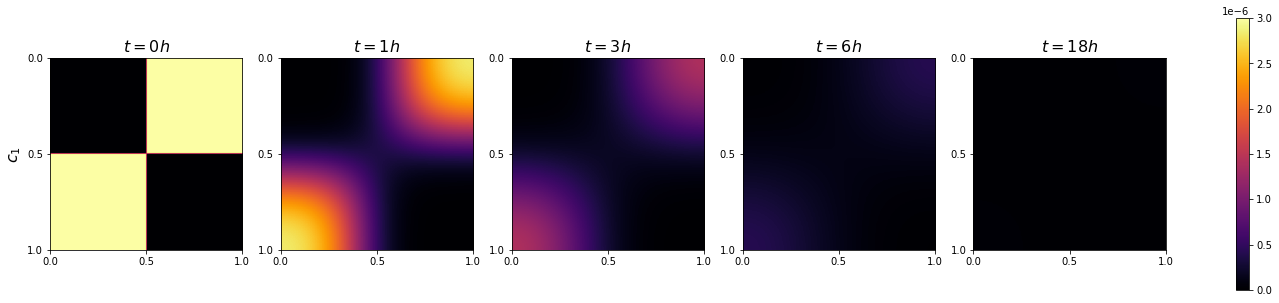
\includegraphics[width=\textwidth]{../paper/assets/example-0.png} \\
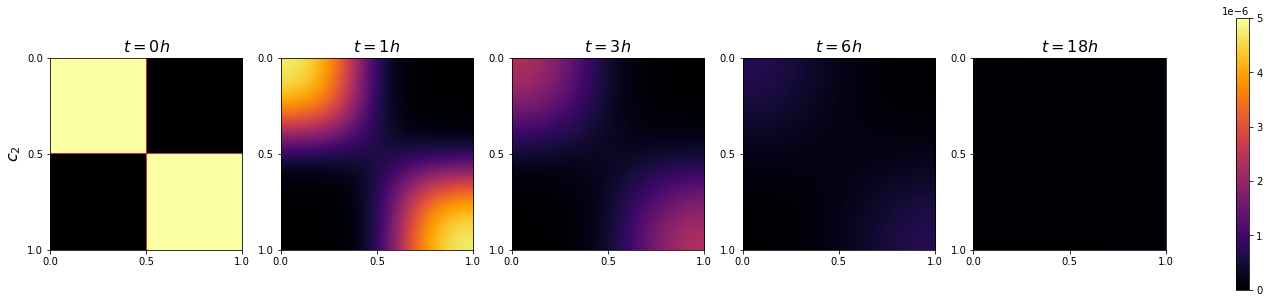
\includegraphics[width=\textwidth]{../paper/assets/example-1.png} \\
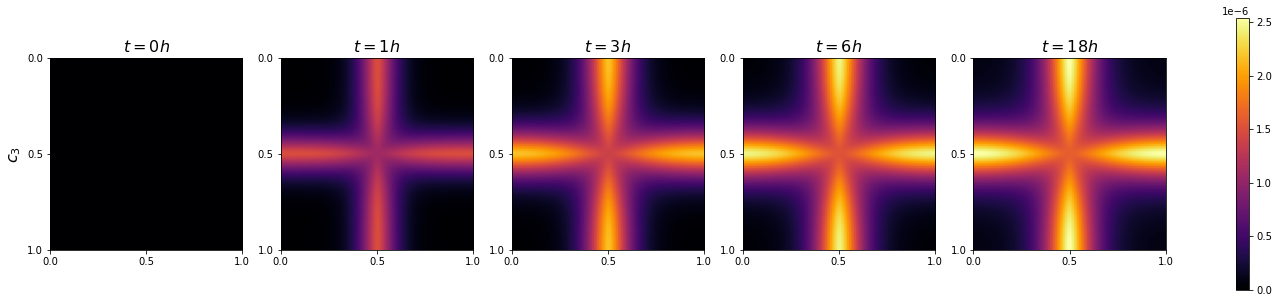
\includegraphics[width=\textwidth]{../paper/assets/example-2.png}
\label{result-example}
\end{figure}

\newpage
\subsection{Programos korektiškumo tikrinimas}

\subsubsection*{Korektiškumo tikrinimas bendru atveju}

% Čia galima tikrint kad individualiu ląstelių
% - keičiant dx/dy kiekio per laiką sprendinys vizualiai konverguoja
% - kiekio grafikai per laika medžiagom c1 ir c2 mažėja, o c3 - didėja.
% - jei nustatom reakcijos koeficienta k = 0, kiekis bus pastovus
% Tikrinti rezultatų korektiškumui yra naudojami tie patys duomenys kaip ir rezultatų vaizdavimui. 

Nagrinėjant programos korektiškumą naudosime modelio rezultatų duomenis. Dėl didelės rezultatų dimensijos būtų sunku interpretuoti grafiškai pavaizduotus sprendinio duomenis, kaip \hbox{\ref{result-example}-ame} pavyzdyje, todėl vietoje tokių grafikų, tyrinėsime medžiagų kiekius sistemoje. Galime išskleisti formulę medžiagos kiekiui bendru atveju \eqref{quantity-general} ir gausime formulę diskrečiam atvejui \cite{strangCalculusVolume32016}:
\begin{align}
    q(t) = \int_\Omega c\,dV = \int_0^W \int_0^H c(x, y, t)\,dy\,dx
\end{align}
Pakeičiam dvigubą integralą su dviguba Rymano suma ir gaunam, kad medžiagos $c_m$ kiekis diskrečiu laiko momentu $n$ yra:
\begin{align}
    q_{m, n}= \sum_{i=0}^{N-1}\sum_{j=0}^{M-1} c_{m, i,j}^n \frac{W\cdot H}{N\cdot M} \quad m=1, 2, 3
\end{align}
Norint nustatyti, ar programa veikia korektiškai galima tikrinti, ar mažinant žingsnių dydį, skaitinis sprendinys artėja prie tikrojo sprendinio. Šiuo atveju mažinsime erdvės žingsnius $\Delta x$ ir $\Delta y$. Tai lemia diskretaus tinklelio taškų kiekio padidėjimą, nes egzistuoja atvirkštinė priklausomybė tarp erdvinių žingsnių dydžio ir diskrečių taškų kiekio atitinkamomis ašimis (\ref{meshx}, \ref{meshy}).
\begin{figure}[h!]
    \centering
    \caption{Kompiuterinio modelio rezultatai - medžiagų kiekių priklausomybė nuo laiko. Čia $\tau=3.6\times 10^5$, $D=0.05$, $W = 1$, $H=1$, $k = 1$, $c_0 = 1$, $\Delta t = 1\times 10^{-5}$, $\Delta x$, $\Delta y$ - kintami ir priklauso nuo $N$ bei $M$ }
    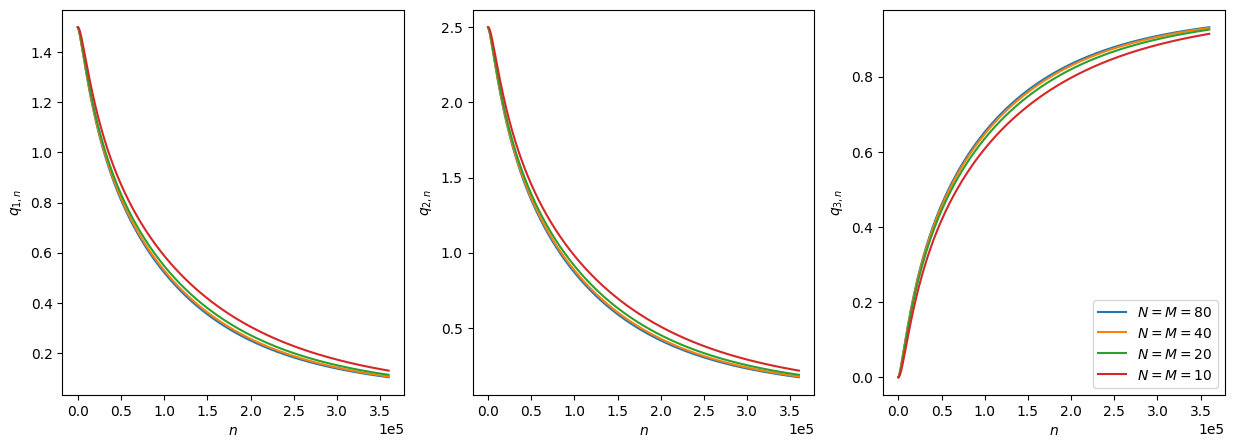
\includegraphics[width=\textwidth]{../assets/space-error-v2.png} \\
    \label{results-space-error}
\end{figure}

\ref{results-space-error}-ame pav. matome, kad eksponentiškai didinant diskrečių taškų skaičių, sprendinių grafikai tolygiai artėja prie sprendinio su didžiausiu tikslumu, darome prielaidą, kad didinant diskrečių taškų skaičių, skaitinis sprendinys konverguoją į tikrąjį sprendinį. Kažkuriuo momentu diskrečios erdvės taškų kiekio didinimas nebeduoda ypatingai didelių rezultato pagerėjimų. Sprendinių grafikuose taip pat galima įžvelgti, kad pirmų dviejų medžiagų kiekiai per laiką griežtai ne mažėja - tai mes teoriškai parodėme \eqref{negative-quantity}, taip, žinoma, yra dėl  medžiagų reakcijos. 

Analogiškai galima būtų fiksuoti erdvinius žingsnius $\Delta x, \Delta y$ ir stebėti kaip keičiasi skaitinis sprendinys mažinant laiko žingsnį $\Delta t$. Dėl priežasčių, kurios vėliau bus akivaizdžios vaizduosime du sprendinius - vienas iš jų gautas pasirinkus $\Delta t$ pagal \eqref{numerical-stability-condition}, o kitam paimta konkreti reikšmė $\Delta t = 10^{-4}$.

\begin{figure}[h!]

\centering

\caption{Kompiuterinio modelio rezultatai - medžiagų kiekių priklausomybė nuo laiko. Čia $\tau=3.6\times 10^5$, $D=0.05$, $W = 1$, $H=1$, $k = 1$, $c_0 = 1$, $\Delta x = \Delta y = 79^{-1}$}

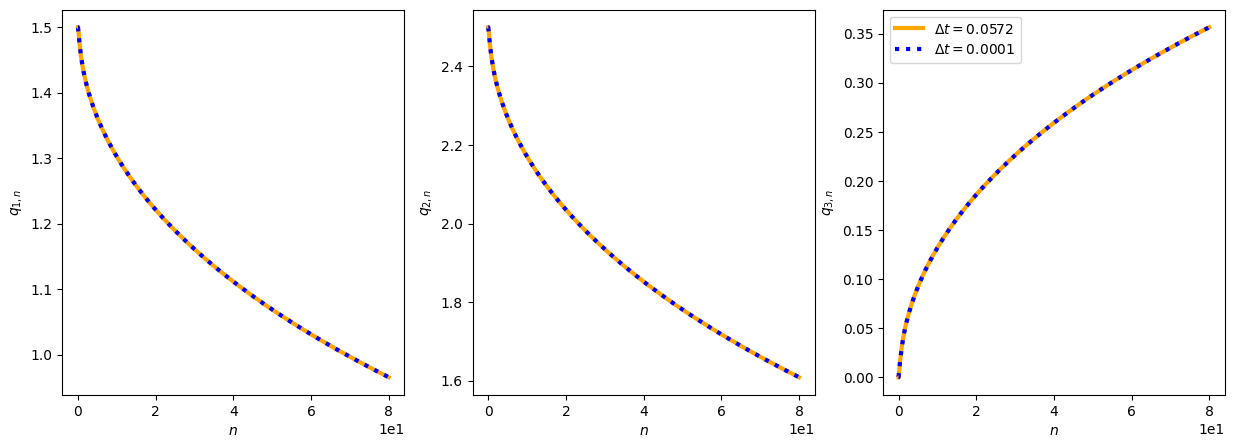
\includegraphics[width=\textwidth]{../assets/time-error-2.png}

\label{time-error}

\end{figure}

\ref{time-error}-ame pav. matome, kad sprendiniai yra identiški. Laiko žingsnio  $\Delta t$ pasirinkimas pagal \eqref{numerical-stability-condition} yra pakankamai geras ir mažesnių laiko žingsnių pasirinkimas neduoda pastebimai tikslesnių rezultatų.

\subsubsection*{Korektiškumo tikrinimas kai vyksta tik difuzija}

Jei reakcijos koeficientas būtų lygus nuliui, vienintelis sistemoje vykstantis procesas būtų pirmų dviejų medžiagų difuzija. Jei skaitinis modelis veikia korektiškai, rezultatuose turėtų būti galima matyti, kad difuzijos metu medžiagos kiekis sistemoje nekinta, tai teoriškai parodėme skyriuje apie skaitinį stabilumą \eqref{no-q-change}.

\newpage

\begin{figure}[h!]
    \centering
    \caption{Kompiuterinio modelio rezultatai - medžiagų kiekių priklausomybė nuo laiko, kai reakcija nevyksta. $D = 0.05$, $W = 1$, $H = 1$, $\Delta x = \frac{1}{79}$, $\Delta y = \frac{1}{79}$, $k = 0$, $c_0 = 1$, $\Delta t = 1\times 10^{-5}$ }
    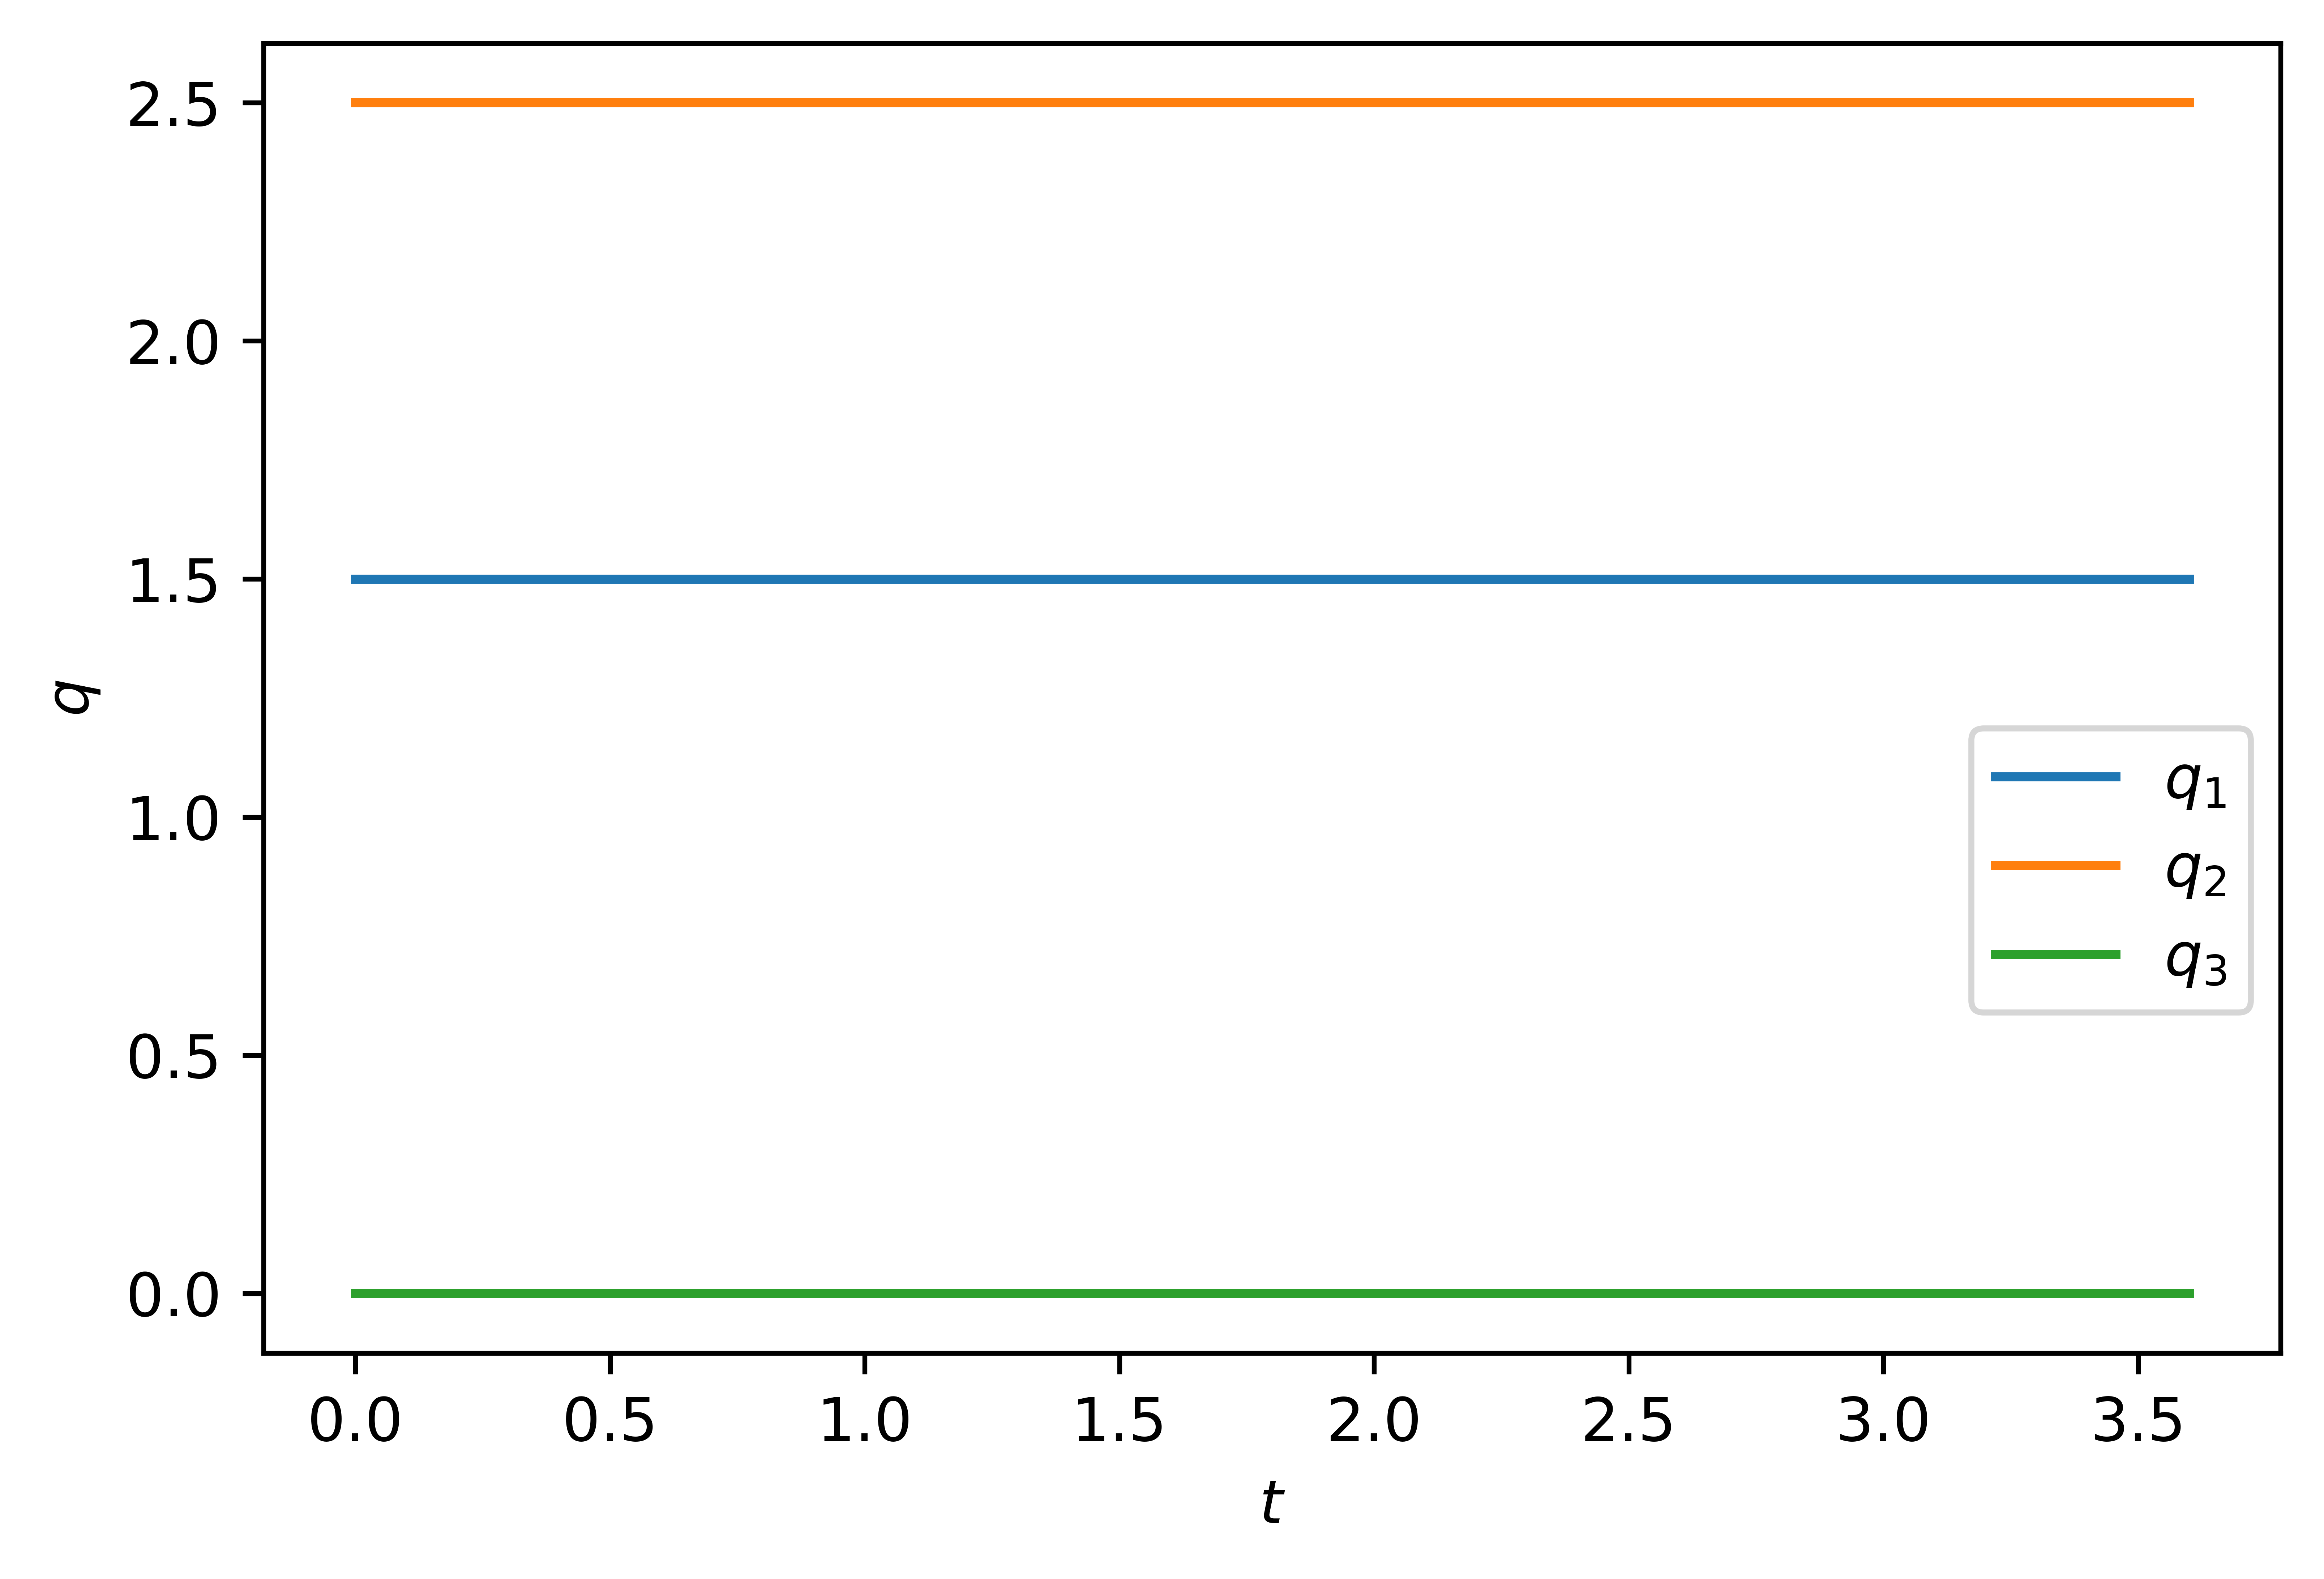
\includegraphics[width=0.5\textwidth]{../assets/no-reaction.png}
    \label{no-reaction}
\end{figure}

\ref{no-reaction}-ame pavyzdyje kompiuterinės programos rezultatai yra būtent tokie, kokių tikėjomės, tačiau iš šio grafiko negalime užtikrinti, kad simuliacijoje išvis kažkas vyksta. Norint patikrinti, ar medžiagos difunduoja korektiškai galime pabandyti pavaizduoti medžiagų kiekį visoje srityje $\Omega$ kaip rezultatų pavyzdyje \eqref{result-example}.

\begin{figure}[h!]
\centering
\caption{Kompiuterinio modelio rezultato pavyzdys, kai vyksta tik difuzija. $D = 0.05$, $W = 1$, $H = 1$, $\Delta x = \frac{1}{79}$, $\Delta y = \frac{1}{79}$, $k = 0$, $c_0 = 1$, $\Delta t = 1\times 10^{-5}$ }
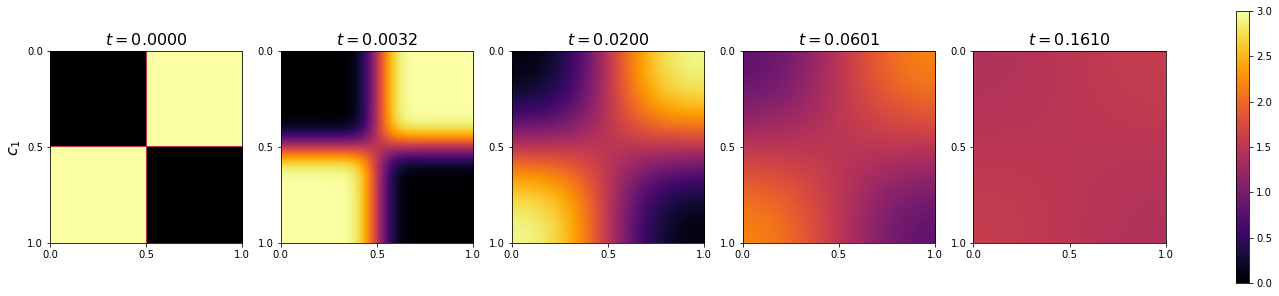
\includegraphics[width=\textwidth]{../assets/only-diffusion-c1.png} \\
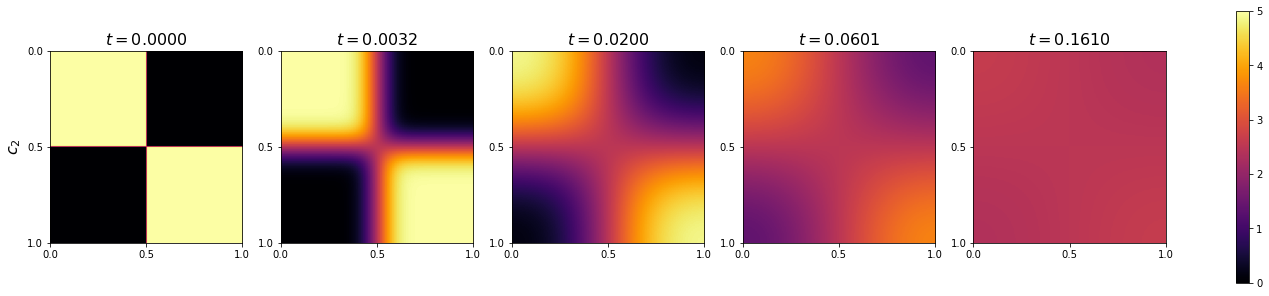
\includegraphics[width=\textwidth]{../assets/only-diffusion-c2.png}
\label{only-diffusion}
\end{figure}

Čia akivaizdžiai galime matyti, kad medžiagų difuzija vyksta ir einant laikui medžiagos tolygiai pasiskirsto po erdvę.


